\PassOptionsToPackage{unicode=true}{hyperref} % options for packages loaded elsewhere
\PassOptionsToPackage{hyphens}{url}
%
\documentclass[ignorenonframetext,]{beamer}
\usepackage{pgfpages}
\setbeamertemplate{caption}[numbered]
\setbeamertemplate{caption label separator}{: }
\setbeamercolor{caption name}{fg=normal text.fg}
\beamertemplatenavigationsymbolsempty
% Prevent slide breaks in the middle of a paragraph:
\widowpenalties 1 10000
\raggedbottom
\setbeamertemplate{part page}{
\centering
\begin{beamercolorbox}[sep=16pt,center]{part title}
  \usebeamerfont{part title}\insertpart\par
\end{beamercolorbox}
}
\setbeamertemplate{section page}{
\centering
\begin{beamercolorbox}[sep=12pt,center]{part title}
  \usebeamerfont{section title}\insertsection\par
\end{beamercolorbox}
}
\setbeamertemplate{subsection page}{
\centering
\begin{beamercolorbox}[sep=8pt,center]{part title}
  \usebeamerfont{subsection title}\insertsubsection\par
\end{beamercolorbox}
}
\AtBeginPart{
  \frame{\partpage}
}
\AtBeginSection{
  \ifbibliography
  \else
    \frame{\sectionpage}
  \fi
}
\AtBeginSubsection{
  \frame{\subsectionpage}
}
\usepackage{lmodern}
\usepackage{amssymb,amsmath}
\usepackage{ifxetex,ifluatex}
\usepackage{fixltx2e} % provides \textsubscript
\ifnum 0\ifxetex 1\fi\ifluatex 1\fi=0 % if pdftex
  \usepackage[T1]{fontenc}
  \usepackage[utf8]{inputenc}
  \usepackage{textcomp} % provides euro and other symbols
\else % if luatex or xelatex
  \usepackage{unicode-math}
  \defaultfontfeatures{Ligatures=TeX,Scale=MatchLowercase}
\fi
% use upquote if available, for straight quotes in verbatim environments
\IfFileExists{upquote.sty}{\usepackage{upquote}}{}
% use microtype if available
\IfFileExists{microtype.sty}{%
\usepackage[]{microtype}
\UseMicrotypeSet[protrusion]{basicmath} % disable protrusion for tt fonts
}{}
\IfFileExists{parskip.sty}{%
\usepackage{parskip}
}{% else
\setlength{\parindent}{0pt}
\setlength{\parskip}{6pt plus 2pt minus 1pt}
}
\usepackage{hyperref}
\hypersetup{
            pdfborder={0 0 0},
            breaklinks=true}
\urlstyle{same}  % don't use monospace font for urls
\newif\ifbibliography
\setlength{\emergencystretch}{3em}  % prevent overfull lines
\providecommand{\tightlist}{%
  \setlength{\itemsep}{0pt}\setlength{\parskip}{0pt}}
\setcounter{secnumdepth}{0}

% set default figure placement to htbp
\makeatletter
\def\fps@figure{htbp}
\makeatother

\usepackage[british]{babel}
\usepackage{graphicx,hyperref,url}
\usepackage{fontawesome}
\usepackage{hyperref}
\usepackage{adjustbox}
\hypersetup{colorlinks=true,allcolors=blue}

\usetheme{metropolis}
\title{Computationally reproducible research}
\subtitle{Leveraging reproducibility tools in laboratory-based research}
\date{September 18, 2018}

\author[Anderson]{
  Brooke Anderson, Colorado State University \\
  Department of Environmental \& Radiological Health Sciences \\ \\
  {\small \faEnvelope: \url{brooke.anderson@colostate.edu}} \\
  {\small \faTwitter: \href{www.twitter.com/gbwanderson}{@gbwanderson}} \\
  {\small \faGithub:  \url{github.com/geanders}} \\ 
  }

\date{}

\begin{document}

\begin{frame}
  \titlepage
\end{frame}

\begin{frame}{Objectives}
\protect\hypertarget{objectives}{}

The objectives for this talk are:

\begin{enumerate}
\tightlist
\item
  Clarify the principle and requirements for \textbf{reproducible
  research}, from a computational standpoint.
\item
  Outline some guidelines for \textbf{recording experimental data} in a
  way that facilitates computationally reproducible research, based on
  two recent papers:

  \begin{itemize}
  \tightlist
  \item
    Broman and Woo (2018) Data Organization in Spreadsheets, \emph{The
    American Statistician}, 72:1, 2--10, DOI:
    10.1080/00031305.2017.1375989
  \item
    Ellis and Leek (2018) How to Share Data for Collaboration, \emph{The
    American Statistician}, 72:1, 53--57, DOI:
    10.1080/00031305.2017.1375987
  \end{itemize}
\end{enumerate}

\end{frame}

\hypertarget{objective-1-clarify-the-principle-and-requirements-for-reproducible-research-from-a-computational-standpoint.}{%
\section{Objective 1: Clarify the principle and requirements for
reproducible research, from a computational
standpoint.}\label{objective-1-clarify-the-principle-and-requirements-for-reproducible-research-from-a-computational-standpoint.}}

\begin{frame}{Reproducible research}
\protect\hypertarget{reproducible-research}{}

\begin{center}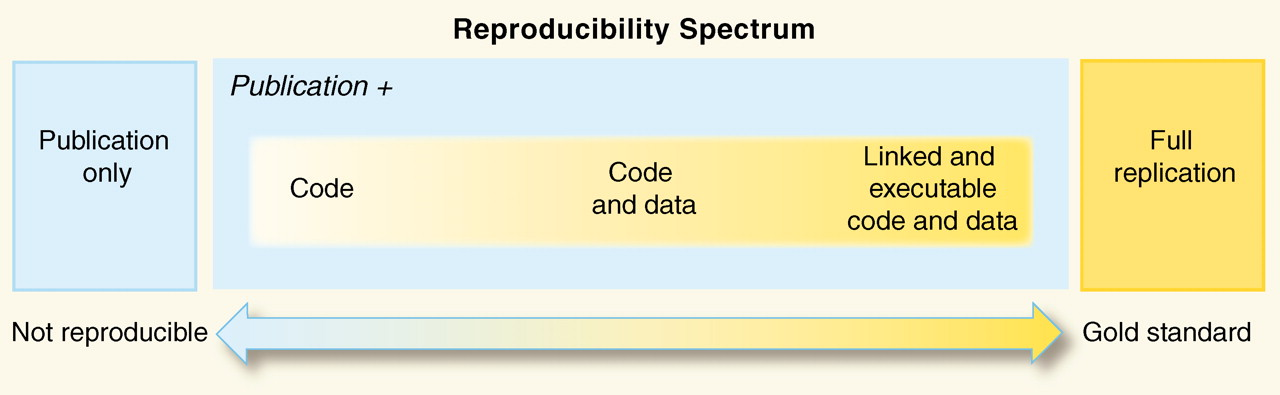
\includegraphics[width=\textwidth]{figures/peng_reproducible} \end{center}

\vspace{-0.4cm}

\scriptsize Source: Peng (2011) Reproducible Research in Computational
Science, \emph{Science}, 334:6060, 1226--1227, DOI:
10.1126/science.1213847

\bigskip

\normalsize Computationally \textbf{reproducible research} is research
for which another person could take the published materials and recreate
the same results from the same raw data.

\end{frame}

\begin{frame}{Reproducible research}
\protect\hypertarget{reproducible-research-1}{}

\begin{columns}

\begin{column}{0.5\textwidth}
\begin{centering}
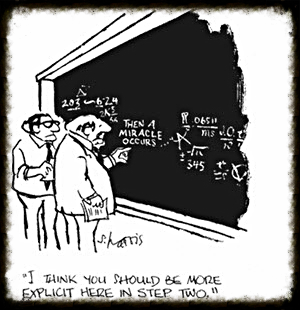
\includegraphics[width=\textwidth]{figures/sidney_harris_new_yorker.png}
\end{centering} \\
\vspace{-0.1cm}
\scriptsize Source: Sidney Harris, The New Yorker
\end{column}

\begin{column}{0.5\textwidth}
\small
To make research computationally reproducible, full instructions should be available describing how you: 

\begin{itemize}
\item Did any cleaning, pre-processing, or reformatting of the \textbf{raw data} (i.e., the data directly recorded for an experiment or output by laboratory equipment)
\item Analyzed the \textbf{processed data} to generate figures, tables, and other research results
\end{itemize}

\textbf{Code scripts} are an excellent way to record this information.

\end{column}

\end{columns}

\end{frame}

\begin{frame}{Common ``black boxes'' in laboratory-based research}
\protect\hypertarget{common-black-boxes-in-laboratory-based-research}{}

\begin{center}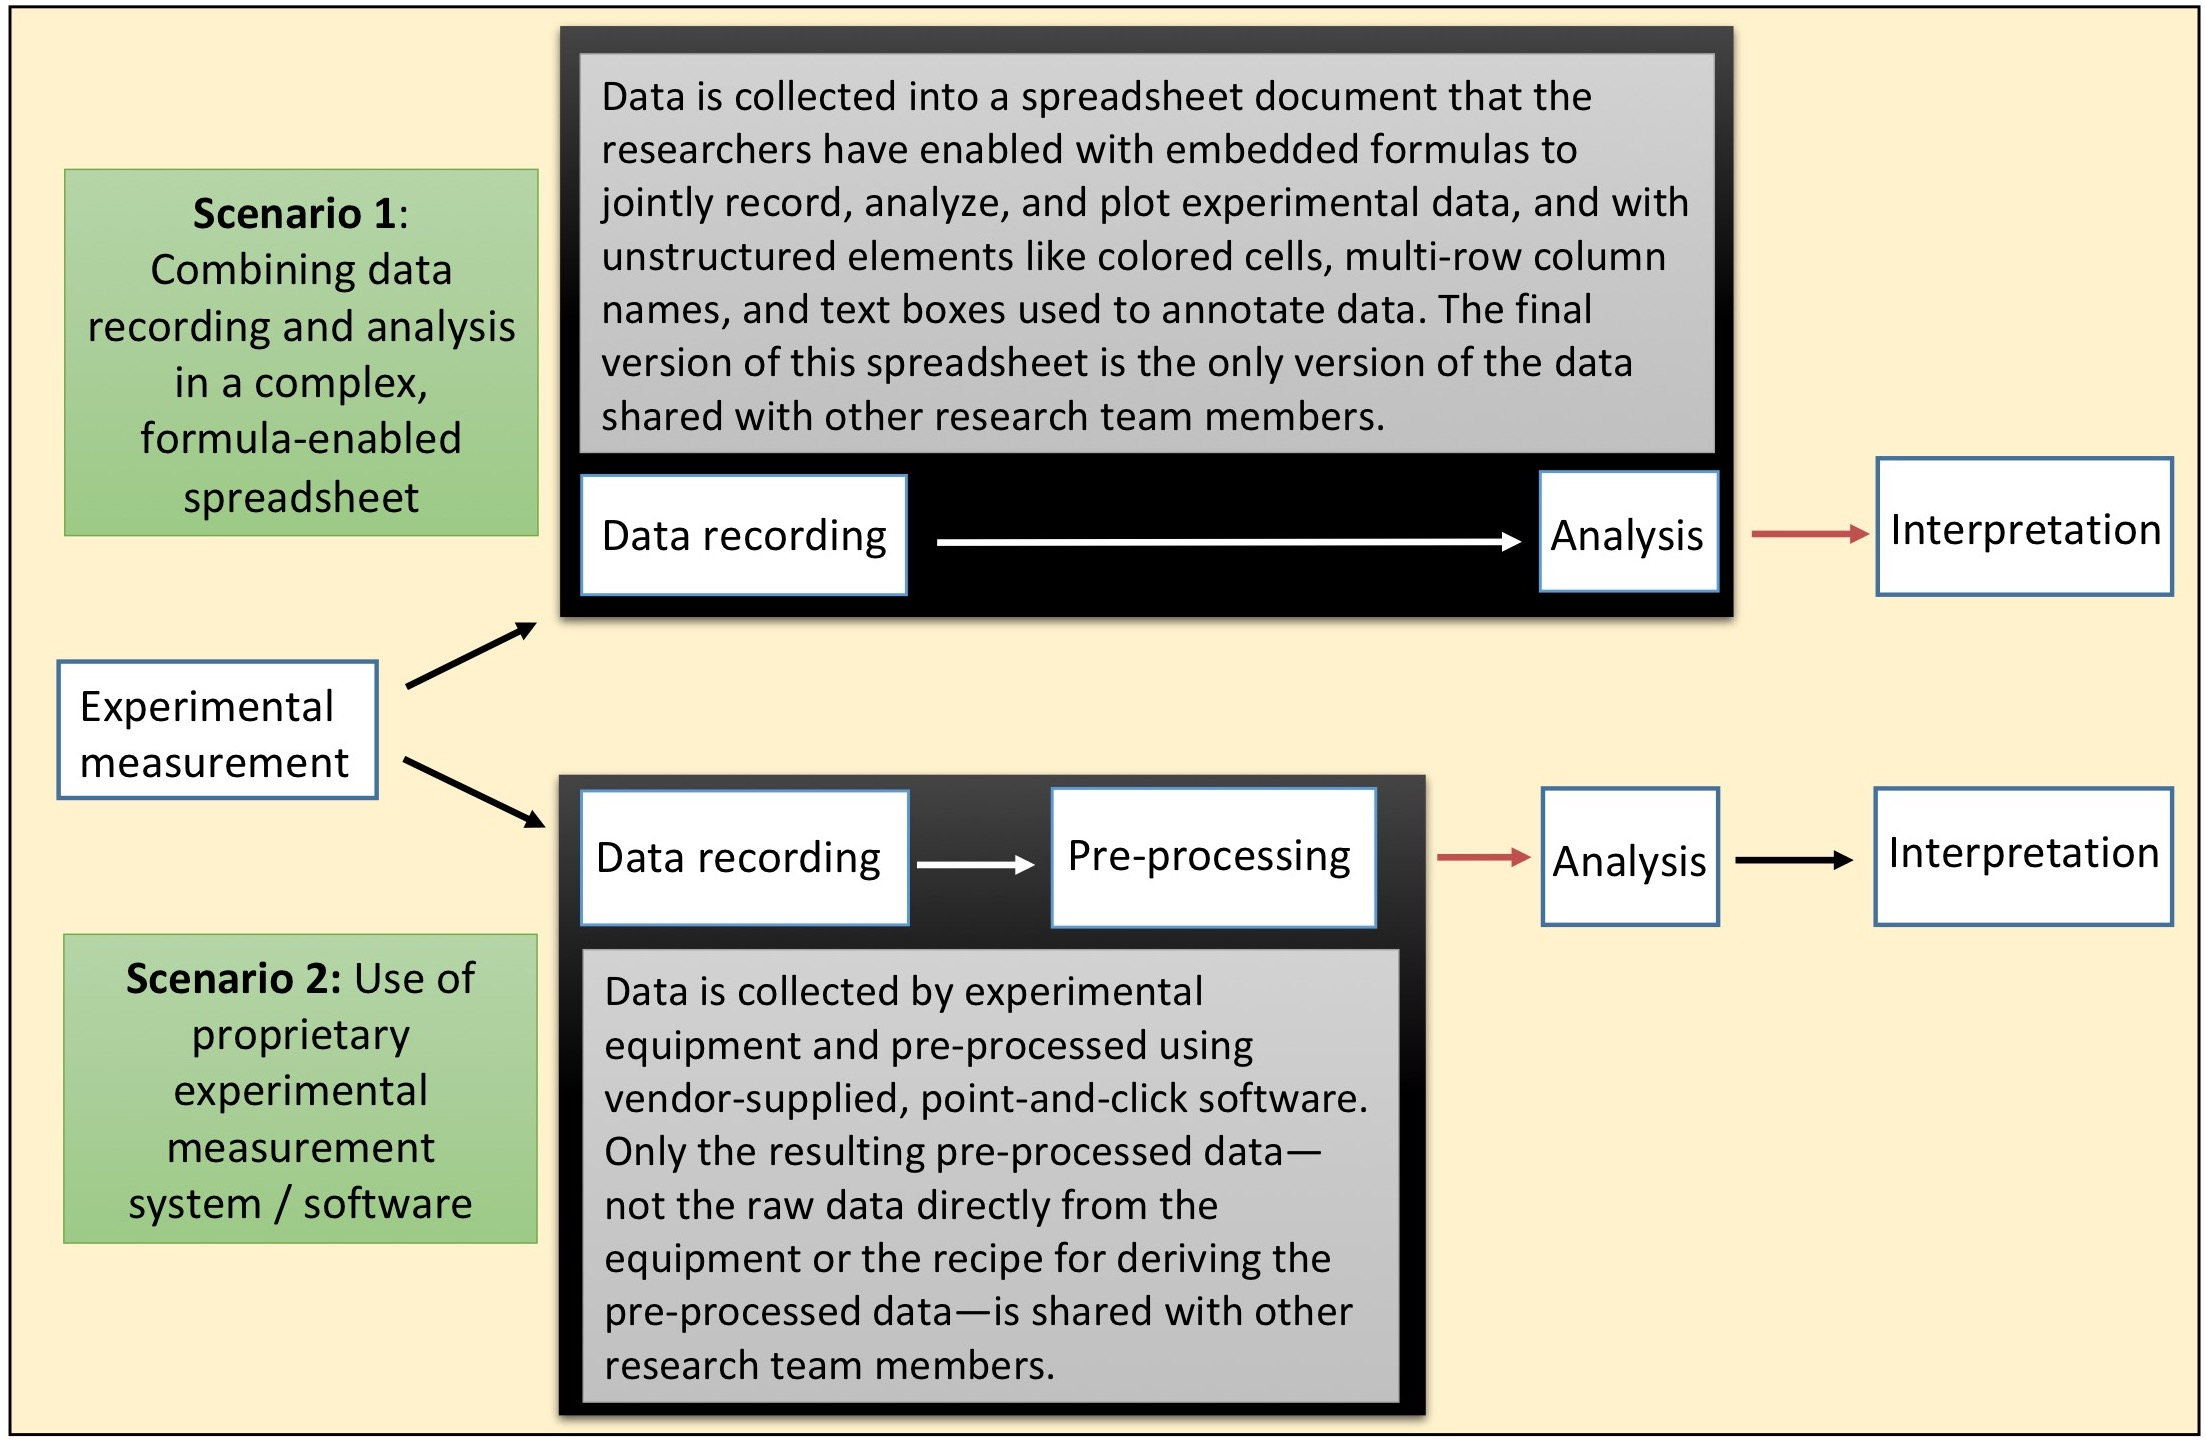
\includegraphics[width=0.9\textwidth]{figures/existing_blackboxes} \end{center}

\small

We identified two common \textbf{black boxes} in laboratory-based
research, where the research steps are often neither
\textbf{transparent} nor \textbf{reproducible}.

\end{frame}

\begin{frame}{``Co-benefits'' of reproducible research}
\protect\hypertarget{co-benefits-of-reproducible-research}{}

\begin{center}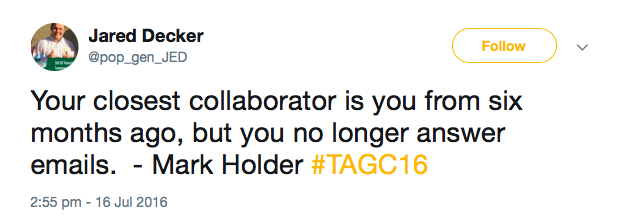
\includegraphics[width=0.8\textwidth]{figures/own_worst_collaborator} \end{center}

\vspace{-0.4cm}

\scriptsize Source: Twitter, @pop\_gen\_JED

\bigskip

\normalsize Meeting the standards of reproducibility can have many
co-benefits for a research lab, including \textbf{increasing efficiency}
of research and \textbf{sharing data pre-processing and analysis
techniques} across laboratory members.

\end{frame}

\hypertarget{objective-2-outline-some-guidelines-for-recording-experimental-data-in-a-way-that-facilitates-computationally-reproducible-research}{%
\section{Objective 2: Outline some guidelines for recording experimental
data in a way that facilitates computationally reproducible
research}\label{objective-2-outline-some-guidelines-for-recording-experimental-data-in-a-way-that-facilitates-computationally-reproducible-research}}

\begin{frame}{Record data in ``rectangular'' formats}
\protect\hypertarget{record-data-in-rectangular-formats}{}

\begin{center}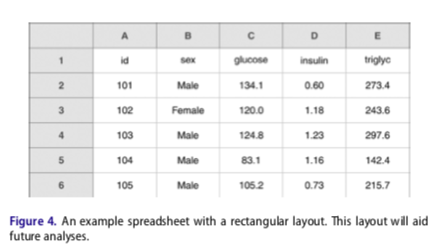
\includegraphics[width=0.8\textwidth]{figures/rectangular_data} \end{center}

\vspace{-0.4cm}

\scriptsize Source: Broman and Woo, 2018

\bigskip

\small \textbf{Rectangular format}: One unit of observation per
spreadsheet; one row for each study observation (e.g., study subject,
time point); one column for each variable being measured; no empty
boxes.

\end{frame}

\begin{frame}{Non-``rectangular'' formats}
\protect\hypertarget{non-rectangular-formats}{}

\begin{center}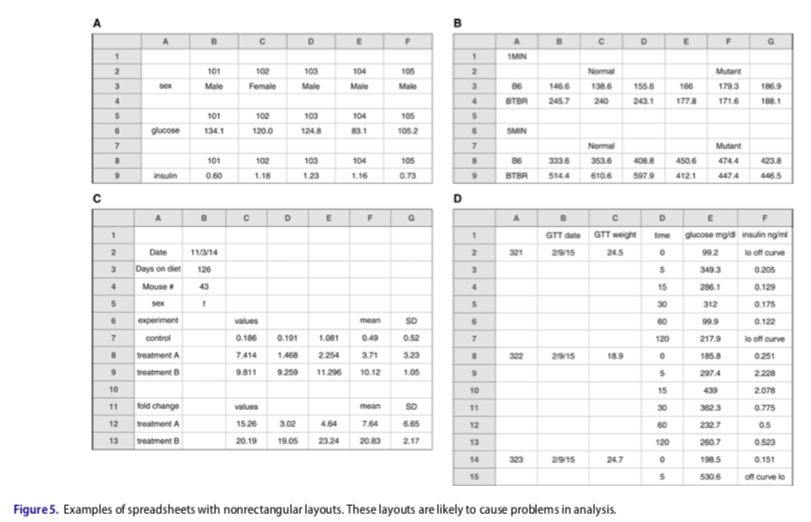
\includegraphics[width=\textwidth]{figures/non_rectangular_data} \end{center}

\vspace{-0.4cm}

\scriptsize Source: Broman and Woo, 2018

\small These may be \textbf{human-readable}, but are much less
\textbf{computer-readable}.

\end{frame}

\begin{frame}{Think in terms of ``plain text'' file formats}
\protect\hypertarget{think-in-terms-of-plain-text-file-formats}{}

\begin{center}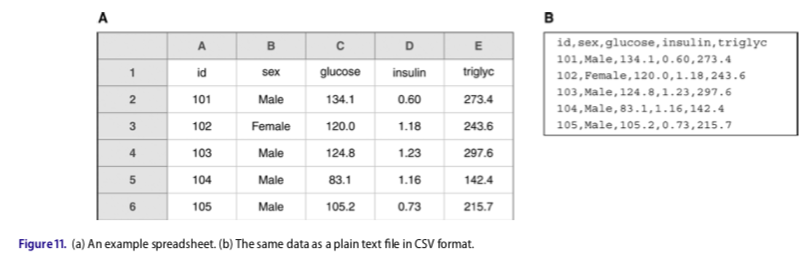
\includegraphics[width=\textwidth]{figures/plain_text_format} \end{center}

\vspace{-0.4cm}

\scriptsize Source: Broman and Woo, 2018

\medskip

\normalsize Ideally, the data recording format should be something that
could be set up as within a \textbf{plain text file format}, like a
comma-separated values format (.csv).

\end{frame}

\begin{frame}{Avoid cell formatting}
\protect\hypertarget{avoid-cell-formatting}{}

\begin{center}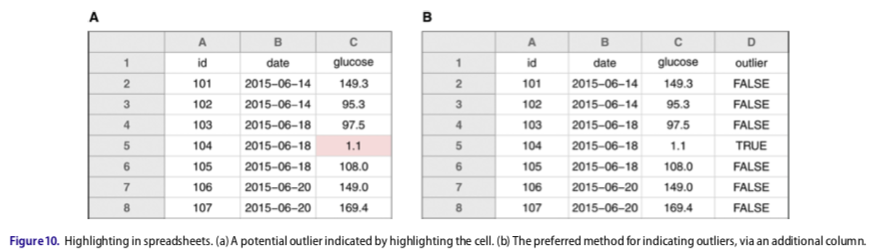
\includegraphics[width=\textwidth]{figures/cell_formatting} \end{center}

\vspace{-0.4cm}

\scriptsize Source: Broman and Woo, 2018

\medskip

\normalsize Any time you use \textbf{highlighting} or other forms of
cell formatting in a spreadsheet, you will lose the information when you
read the data into R or Python. Similarly, avoid adding
\textbf{text boxes} or \textbf{embedded formulas} to spreadsheets used
for data recording.

\end{frame}

\begin{frame}{Be careful in naming columns}
\protect\hypertarget{be-careful-in-naming-columns}{}

\begin{center}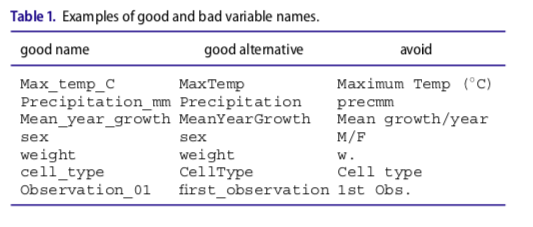
\includegraphics[width=\textwidth]{figures/column_names} \end{center}

\vspace{-0.4cm}

\scriptsize Source: Broman and Woo, 2018

\medskip

\normalsize Make sure that column names do not have \textbf{spaces},
\textbf{mathematical symbols}, or \textbf{other special characters}.

\end{frame}

\begin{frame}{More guidelines}
\protect\hypertarget{more-guidelines}{}

\begin{center}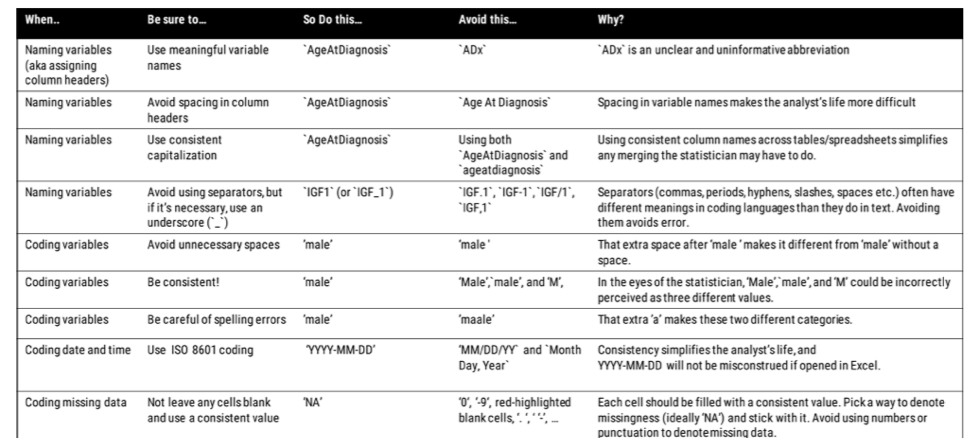
\includegraphics[width=\textwidth]{figures/when_be_sure_to} \end{center}

\vspace{-0.4cm}

\scriptsize Source: Ellis and Leek, 2018

\normalsize \textbf{Similar and additional guidelines} are outlined in
Ellis and Leek, 2018.

\end{frame}

\end{document}
